\chapter{Singular Homology}
\section*{The Eilenberg-Steenrod Axioms}

\begin{definition}[The Eilenberg-Steenrod Axioms]
	A \bld{homology theory} consist of two sequences $(\mathcal{H}_n)_{n \in \omega}$ and $(\delta_n)_{n \in \omega}$, where for each $n \in \omega$, $\mathcal{H}_n : \mathsf{Top}^2 \to \mathsf{AbGrp}$ is a functor and $\delta_n : \mathcal{H}_n \Rightarrow \mathcal{H}_{n - 1} \circ R$ if $n > 0$ and $\delta_0 : \mathcal{H}_0 \Rightarrow 0$ is a natural transformation, with $R : \mathsf{Top}^2 \to \mathsf{Top}^2$ defined by $R(X,A) := (A,\varnothing)$, and subject to the following axioms:
	\begin{itemize}[wide = 0pt]
		\item \textbf{The Exact Sequence Axiom.} Let $(X,A) \in \ob(\mathsf{Top}^2)$. Then there exists a long exact sequence
			\begin{equation*}
				\begin{tikzcd}[column sep=7ex]
					\cdots \arrow[r] & \mathcal{H}_n(A) \arrow[r,"\mathcal{H}_n(\iota_A)"] & \mathcal{H}_n(X) \arrow[r,"\mathcal{H}_n(\iota_X)"] & \mathcal{H}_n(X,A) \arrow[r,"\delta_n"] & \mathcal{H}_{n - 1}(A) \arrow[r] & \cdots
				\end{tikzcd}
			\end{equation*}
			\noindent where $\iota_A : (A,\varnothing) \hookrightarrow (X,\varnothing)$ and $\iota_X : (X,\varnothing) \hookrightarrow (X,A)$ denote inclusions.
		\item \textbf{The Dimension Axiom.} Let $\ast$ be the terminal object in $\mathsf{Top}$. Then $\mathcal{H}_0(\ast) \cong \mathbb{Z}$ and $\mathcal{H}_n(\ast) = 0$ for all $n \in \omega$, $n > 0$. 
	\end{itemize}
\end{definition}


\section*{Construction of the Singular Homology Functor}

Aim of this section is to construct for each $n \in \omega$ a functor $H_n : \mathsf{Top} \to \mathsf{AbGrp}$, called the \textit{$n$-th singular homology functor}.

\subsection*{Free Abelian Groups}

\begin{proposition}
	\label{prop:F_set_abgrp}
	The forgetful functor $U : \mathsf{AbGrp} \to \mathsf{Set}$ admits a left adjoint.	
\end{proposition}

\begin{proof}
	We have to construct a functor $F : \mathsf{Set} \to \mathsf{AbGrp}$. Let $S$ be a set. Define 
	\begin{equation*}
		F(S) := \cbr[1]{f \in \mathbb{Z}^S : \supp f \text{ is finite}}.
	\end{equation*}
	Equipped with pointwise addition, $F(S)$ is an abelian group. There is a natural inclusion $\iota : S \hookrightarrow U\del[1]{F(S)}$ sending $x \in S$ to the function taking the value one at $x$ and zero else. Hence we may regard elements of $F(S)$ as formal linear combinations $\sum_{x \in S}m_x x$, where $m_x \in \mathbb{Z}$ for all $x \in S$. On morphisms $f : S \to T$ in $\mathsf{Set}$, define $F(f) : F(S) \to F(T)$ simply by setting $F(f)\del[1]{\sum_{x \in S}m_x x} := \sum_{x \in S}m_x f(x)$.\\	
	Let $G \in \ob(\mathsf{AbGrp})$ be an abelian group and $\varphi \in \mathsf{AbGrp}\del[1]{F(S), G}$ a morphism of groups. Define $\wbar{\varphi} \in \mathsf{Set}\del[1]{S,U(G)}$ by $\wbar{\varphi} := U(\varphi)$. Conversly, if we have $f \in \mathsf{Set}\del[1]{S,U(G)}$, define $\wbar{f} \in \mathsf{AbGrp}\del[1]{F(S),G}$ by $\wbar{f}\del[1]{\sum_{x \in S} m_x x} := \sum_{x \in S} m_x f(x)$. This is well defined since all but finitely many $m_x$ are zero and $G$ is abelian. It is easy to check that $\wbar{f}$ is indeed a morphism of groups. Let $\varphi \in \mathsf{AbGrp}\del[1]{F(S),G}$. Then
	\begin{align*}
		\wbar{\wbar{\varphi}}\del[4]{\sum_{x \in S} m_x x} &= \sum_{x \in S}m_x \wbar{\varphi}(x)\\
		&= \sum_{x \in S} m_x U(\varphi)(x)\\
		&= \sum_{x \in S} m_x \varphi(x)\\
		&= \varphi \del[4]{\sum_{x \in S} m_x x}.
	\end{align*}
	And for $f \in \mathsf{Set}\del[1]{S,U(G)}$ we have that
	\begin{equation*}
		\wbar{\wbar{f}}(x) = U(\wbar{f})(x) = \wbar{f}(x) = f(x). 
	\end{equation*}
	\noindent Hence $\wbar{\wbar{\varphi}} = \varphi$ and $\wbar{\wbar{f}} = f$ and so we have a bijection
	\begin{equation*}
		\mathsf{AbGrp}\del[1]{F(S),G} \cong \mathsf{Set}\del[1]{S,U(G)}.
	\end{equation*}
	The mapping $f \mapsto \wbar{f}$ will be referred to as \bld{extending by linearity}. To check naturality in $S$ and $G$ is left as an exercise.
\end{proof}

\begin{exercise}
	In proposition \ref{prop:F_set_abgrp}, check that $F : \mathsf{Set} \to \mathsf{AbGrp}$ is indeed a functor, called the \bld{free functor from $\mathsf{Set}$ to $\mathsf{AbGrp}$}, and the naturality of the bijection in both arguments. 
\end{exercise}

\begin{definition}[Free Abelian Group]
	Let $F : \mathsf{Set} \to \mathsf{AbGrp}$ be the free functor. For any set $S$, we call $F(S)$ the \bld{free group generated by $S$}.
\end{definition}

\subsection*{Chain Complexes}

\begin{definition}[Chain Complex]
	A \bld{chain complex} is a tuple $(C_\bullet,\partial_\bullet)$ consisting of a sequence $(C_n)_{n \in \mathbb{Z}}$ in $\ob(\mathsf{AbGrp})$ and a sequence $(\partial_n)_{n \in \mathbb{Z}}$ in $\mor(\mathsf{AbGrp})$, called \bld{boundary operators}, such that we have $\partial_{n} \in \mathsf{AbGrp}(C_n,C_{n - 1})$ and $\partial_n \circ \partial_{n + 1} = 0$ for all $n \in \mathbb{Z}$.
\end{definition}

\begin{definition}[Chain Maps]
	Let $(C_\bullet,\partial_\bullet)$ and $(C'_\bullet,\partial'_\bullet)$ be two chain complexes. A \bld{chain map $f_\bullet : C_\bullet \to C'_\bullet$} is a sequence $(f_n)_{n \in \mathbb{Z}}$ in $\mor(\mathsf{AbGrp})$ such that $f_n \in \mathsf{AbGrp}(C_n,C'_n)$ and the diagram
	\begin{equation*}
		\begin{tikzcd}
			C_n \arrow[r,"\partial_n"]\arrow[d,"f_n"'] & C_{n - 1} \arrow[d,"f_{n - 1}"] \\
			C'_n \ar[r,"\partial'_n"'] & C'_{n - 1}
		\end{tikzcd}
	\end{equation*}
	\noindent commutes for all $n \in \mathbb{Z}$.
\end{definition}

\begin{proposition}
	There is a category with objects chain complexes and morphisms chain maps.
	\label{prop:comp}
\end{proposition}

\begin{proof}
	Let $f_\bullet : C_\bullet \to C'_\bullet$ and $g_\bullet : C_\bullet' \to C_\bullet''$ be chain maps. Define a map $g_\bullet \circ f_\bullet$ by $g_n \circ f_n$ for each $n \in \mathbb{Z}$. This defines a chain map. Moreover, for each chain complex $C_\bullet$ define $\id_{C_\bullet}$ by $\id_{C_n}$ for all $n \in \mathbb{Z}$. It is easy to check, that then $\circ$ is associative and the identity laws hold.
\end{proof}

\begin{definition}[$\mathsf{Comp}$]
	The category in \ref{prop:comp} is called the \bld{category of chain complexes} and we refer to it as $\mathsf{Comp}$.
\end{definition}

\begin{theorem}
	There is a functor $\mathsf{Top} \to \mathsf{Comp}$.
	\label{thm:singular_complex}
\end{theorem}

\begin{proof}
	The proof is divided into several steps. Let us denote $C_\bullet : \mathsf{Top} \to \mathsf{Comp}$ for the claimed functor.
	\begin{enumerate}[label = \textit{Step \arabic*:},wide = 0pt, itemsep = 1.5ex]
		\item \textit{Construction of a sequence of abelian groups.} Let $v_0,\dots,v_k \in \mathbb{R}^n$ for some $n,k \in \omega$. We say that $(v_0,\dots,v_k)$ is \bld{affinely independent} if $(v_1 - v_0,\dots, v_k - v_0)$ is linearly independent. We define the \bld{k-simplex spanned by $(v_0,\dots,v_k)$}, written $\sbr[0]{v_0,\dots,v_k}$, to be
			\begin{equation}
				\textstyle{\sbr[0]{v_0,\dots,v_k} := \cbr[1]{\sum_{i = 0}^k s_i v_i : s_i \geq 0 \text{ for all } i = 0,\dots,k \text{ and } \sum_{i = 0}^k s_i = 1}}.
			\end{equation}
			\noindent equipped with the subspace topology. Moreover, we define the \bld{standard $n$-simplex $\Delta^n$} to be the $n$-simplex spanned by $(e_0,\dots,e_n)$ where $e_0 := 0 \in \mathbb{R}^n$ and $(e_1,\dots,e_n)$ is the standard ordered basis of $\mathbb{R}^n$. Let $X \in \ob(\mathsf{Top})$. Define a \bld{singular $n$-simplex in $X$} to be a morphism $\sigma \in \mathsf{Top}(\Delta^n,X)$. Let $n \in \mathbb{Z}$. Define
			\begin{equation}
				C_n(X) := \ccases{F\del[1]{\mathsf{Top}(\Delta^n,X)} & n \geq 0,\\
									0 & n < 0.}
			\end{equation}
			We will call elements of $C_n(X)$ \bld{singular $n$-chains}.
		\item \textit{Construction of boundary operators.} Let $X \in \ob(\mathsf{Top})$ and $\sigma$ a singular $n$-simplex in $X$ for $n \geq 1$. We define $\varphi^n_k : \Delta^{n-1} \to \Delta^n$, called the \bld{$k$-th face map}, to be the unique affine map determined by the vertex map
			\begin{equation*}
				\begin{matrix}
					& \varphi_k^n\\
					e_0 & \mapsto & e_0\\
					\vdots & & \vdots\\
					e_{k - 1} & \mapsto & e_{k - 1}\\
					e_k & \mapsto & e_{k + 1}\\
					\vdots & & \vdots\\
					e_{n - 1} & \mapsto & e_n.
				\end{matrix}
			\end{equation*}
			Explicitely, given $\sum_{i = 0}^{n - 1} s_i e_i \in \Delta^{n - 1}$, we have that (see \cite[152]{lee:topological_manifolds:2011})
			\begin{equation*}
				\varphi_k^n \del[4]{\sum_{i = 0}^{n - 1}s_i e_i} = \sum_{i = 0}^{n - 1}s_i \varphi_k^n(e_i).
			\end{equation*}
			Define now
			\begin{equation}
				\partial \sigma := \sum_{k = 0}^n (-1)^k \sigma \circ \varphi_k^n \in U\del[1]{C_{n - 1}(X)} 
			\end{equation}
			\noindent to be the \bld{boundary of $\sigma$}. Moreover, the \bld{singular boundary operator} is defined to be $\wbar{\partial_n}$ and $\partial_n := 0$ for $n \leq 0$.
		\item \textit{$\partial_n \circ \partial_{n + 1} = 0$ for all $n \in \mathbb{Z}$.} It is enough to consider $n \geq 1$, since $\partial_n \circ \partial_{n + 1} = 0$ holds trivially in the other cases. Let $X \in \ob(\mathsf{Top})$ and $\sigma \in \mathsf{Top}(\Delta^{n+1},X)$. Then we have
			\begin{align*}
				(\partial_n \circ \partial_{n + 1})(\sigma) &= \partial_n \del[4]{\sum_{k = 0}^{n + 1} (-1)^k \sigma \circ \varphi^{n + 1}_k}\\
				&= \sum_{k = 0}^{n + 1} (-1)^k \partial_n\del[1]{\sigma \circ \varphi^{n + 1}_k}\\
				&= \sum_{k = 0}^{n + 1}\sum_{j = 0}^n (-1)^{k + j} \sigma \circ \varphi^{n + 1}_k \circ \varphi^n_j\\
				&= \sum_{0 \leq k \leq j \leq n}(-1)^{k + j} \sigma \circ \varphi^{n + 1}_k \circ \varphi^n_j + \sum_{0 \leq j < k \leq n + 1}(-1)^{k + j} \sigma \circ \varphi^{n + 1}_k \circ \varphi^n_j\\
				&= \sum_{0 \leq j \leq k \leq n}(-1)^{k + j} \sigma \circ \varphi^{n + 1}_j \circ \varphi^n_k + \sum_{0 \leq j <k \leq n + 1}(-1)^{k + j} \sigma \circ \varphi^{n + 1}_k \circ \varphi^n_j\\
				&= \sum_{0 \leq j < k \leq n + 1}\del[1]{(-1)^{k + j - 1} \sigma \circ \varphi^{n + 1}_j \circ \varphi^n_{k - 1} + (-1)^{k + j} \sigma \circ \varphi^{n + 1}_k \circ \varphi^n_j}
			\end{align*}
			Since $\varphi_j^{n + 1} \circ \varphi_{k - 1}^n = \varphi_k^{n + 1} \circ \varphi_j^n$, it follows that
			\begin{equation*}
				\partial_n \circ \partial_{n + 1} = 0.
			\end{equation*}
			Indeed, consider the following chart of vertex maps:
			\begin{equation*}
				\begin{matrix}
					& \varphi_{k - 1}^n & & \varphi_j^{n + 1}\\
					e_0 & \mapsto & e_0 & \mapsto & e_0\\
					\vdots & & \vdots & & \vdots\\
					e_{j - 1} & \mapsto & e_{j - 1} & \mapsto & e_{j - 1}\\
					e_j & \mapsto & e_j & \mapsto & e_{j + 1}\\
					\vdots & & \vdots\\
					e_{k - 1} & \mapsto & e_{k - 1} & \mapsto & e_{k + 1}\\
					e_k & \mapsto & e_{k + 1} & \mapsto & e_{k + 2}\\
					\vdots & & \vdots\\
					e_{n - 1} & \mapsto & e_n & \mapsto & e_{n + 1}
				\end{matrix}
				\qquad\qquad\qquad
				\begin{matrix}
					& \varphi_j^n & & \varphi_k^{n + 1}\\
					e_0 & \mapsto & e_0 & \mapsto & e_0\\
					\vdots & & \vdots & & \vdots\\
					e_{j - 1} & \mapsto & e_{j - 1} & \mapsto & e_{j - 1}\\
					e_j & \mapsto & e_{j + 1} & \mapsto & e_{j + 1}\\
					\vdots & & \vdots\\
					e_{k - 1} & \mapsto & e_k & \mapsto & e_{k + 1}\\
					e_k & \mapsto & e_{k + 1} & \mapsto & e_{k + 2}\\
					\vdots & & \vdots\\
					e_{n - 1} & \mapsto & e_n & \mapsto & e_{n + 1}
				\end{matrix}.
			\end{equation*}
		\item \textit{Construction of chain maps.} Let $X,Y \in \ob(\mathsf{Top})$ and $f \in \mathsf{Top}(X,Y)$. For $n \geq 0$, define $f_n^\# : \mathsf{Top}(\Delta^n,X) \to U\del[1]{C_n(Y)}$ by $f^\# := f \circ \sigma$. Extending this map by linearity yields a homomorphism $f_n^\# : C_n(X) \to C_n(Y)$. Moreover, set $f_n^\# := 0$ for $n < 0$. Let $n \geq 1$ and $\sigma \in \mathsf{Top}(\Delta^n,X)$. Then on one hand we have
			\begin{equation*}
				(f_{n - 1}^\# \circ \partial_n)(\sigma) = f^\#_{n - 1}\del[4]{\sum_{k = 0}^n (-1)^k \sigma \circ \varphi^n_k} = \sum_{k = 0}^n (-1)^k f \circ \sigma \circ \varphi^n_k
			\end{equation*}
			\noindent and on the other
			\begin{equation*}
				(\partial_n \circ f^\#_n)(\sigma) = \partial_n(f \circ \sigma) = \sum_{k = 0}^n (-1)^k f \circ \sigma \circ \varphi^n_k.
			\end{equation*}
	\end{enumerate}
	Checking, that $C_\bullet$ is indeed a functor is left as an exercise.
\end{proof}

\begin{exercise}
	Show that $C_\bullet : \mathsf{Top} \to \mathsf{Comp}$ is a functor.
\end{exercise}

\subsection*{The Homology Functor}
\begin{proposition}
	For each $n \in \mathbb{Z}$ there exists a functor $\mathsf{Comp} \to \mathsf{AbGrp}$.
	\label{prop:homology_functor}
\end{proposition}

\begin{proof}
	Let $(C_\bullet,\partial_\bullet)$ be a chain complex. Let $x \in \im \partial_{n + 1}$. Hence there exists $y \in C_{n + 1}$ such that $x = \partial_{n + 1}y$. But then $\partial_nx = (\partial_n \circ \partial_{n + 1})(y) = 0$ and thus $\im \partial_{n + 1} \subseteq \ker \partial_n$. Define
	\begin{equation*}
		H_n(C_\bullet,\partial_\bullet) := \frac{\ker \partial_n}{\im \partial_{n + 1}} \in \ob(\mathsf{AbGrp}).
	\end{equation*}
	Let $(C_\bullet',\partial_\bullet')$ be a chain complex and $f_\bullet : C_\bullet \to C_\bullet'$ a chain map. Then $f_n(\ker\partial_n) \subseteq \ker \partial_n'$. Indeed, if $y \in f_n(\ker\partial_n)$, there exists $x \in \ker\partial_n$, such that $y = f_n(x)$. Since $f_\bullet$ is a chain map, we thus have $\partial_n'y = (\partial_n' \circ f_n)(x) = (f_{n - 1} \circ \partial_n)(x) = 0$. Moreover, we have that $\im \partial_{n + 1} \subseteq \ker \pi_n' \circ f_n$, where $\pi_n' : \ker \partial_n' \to H_n(C_\bullet',\partial_\bullet')$ is the usual projection. Indeed, if $y \in \im \partial_{n + 1}$, we find $x \in C_{n + 1}$, such that $y = \partial_{n + 1}x$. Since again $f_\bullet$ is a chain map, we have that $f_ny = (f_n \circ \partial_{n + 1})(x) = (\partial_{n + 1}' \circ f_{n + 1})(x) \in \im \partial_{n + 1}' = \ker \pi_n'$. Hence $\pi_n' \circ f_n$ factors uniquely through $\pi_n : \ker \partial_n \to H_n(C_\bullet,\partial_\bullet)$. Define $H_n(f_\bullet)$ to be this map. 
\end{proof}

\begin{remark}
	Let $(C_\bullet,\partial_\bullet)$ be a chain complex and $n \in \mathbb{Z}$. Then we will write $\langle x \rangle$ for an element in $H_n(C_\bullet,\partial_\bullet)$, the so-called \emph{homology class}. Hence if $(C_\bullet',\partial_\bullet')$ is another chain complex and $f_\bullet : C_\bullet \to C_\bullet'$ a chain map, then $H_n(f)\langle c \rangle = \langle f_nc\rangle$. 
\end{remark}

\begin{definition}[Cycles and Boundaries]
	Let $(C_\bullet,\partial_\bullet)$ be a chain complex and $n \in \mathbb{Z}$. Then elements of $\ker \partial_n$ are called \bld{$n$-cycles} and elements of $\im \partial_{n + 1}$ are called \bld{$n$-boundaries}.
\end{definition}

\begin{definition}[Homology Functor]
	Let $n \in \mathbb{Z}$ and $H_n : \mathsf{Comp} \to \mathsf{AbGrp}$ be the functor defined in proposition \ref{prop:homology_functor}. We call $H_n$ the \bld{n-th homology functor}.
\end{definition}

\begin{definition}[Singular Homology Functor]
	Let $n \in \mathbb{Z}$. The composition 
	\begin{equation}
		H_n \circ C_\bullet : \mathsf{Top} \to \mathsf{AbGrp}
	\end{equation}
	\noindent of the singular chain complex functor $C_\bullet$ in theorem \ref{thm:singular_complex} and the $n$-th homology functor of proposition \ref{prop:homology_functor} is called the \bld{$n$-th singular homology functor}, written $H^{\mathrm{sing}}_n$.
\end{definition}

\begin{remark}
	For notational purposes we will often refer to the functor $H_n^{\mathrm{sing}}$ simply as $H_n$.
\end{remark}

%%%%%%%%%%%%%%%%%%%%%%%%%%%%%%%%%%%%%%%%%%%%%%%%%%%%%%%%%%%%%%%%%%%%%%%%%%%%%%%%%%%%%%%%%%%%%%%%%%%%%%%%%%%%%
%Relative and Reduced Homology																				%
%%%%%%%%%%%%%%%%%%%%%%%%%%%%%%%%%%%%%%%%%%%%%%%%%%%%%%%%%%%%%%%%%%%%%%%%%%%%%%%%%%%%%%%%%%%%%%%%%%%%%%%%%%%%%
\subsection*{Relative Homology}
\begin{definition}[Subcomplex]
	Let $(C_\bullet,\partial_\bullet)$ be a chain complex. A \bld{subcomplex} of $(C_\bullet,\partial_\bullet)$ is a chain complex $(C_\bullet',\partial_\bullet')$, such that $C_n' \subseteq C_n$ for all $n \in \mathbb{Z}$ and that $\iota : C_\bullet' \to C_\bullet$ defined by $\iota_n : C_n' \hookrightarrow C_n$ for all $n \in \mathbb{Z}$, is a chain map.
\end{definition}

\begin{definition}[Quotient Complex]
	Let $(C_\bullet',\partial_\bullet')$ be a subcomplex of $(C_\bullet,\partial_\bullet)$. Then define the \bld{quotient complex}, written $C_\bullet/C_\bullet'$, by setting
	\begin{equation*}
		(C_\bullet/C_\bullet')_n := C_n/C_n' \qquad \text{and} \qquad \partial_n := C_n/C_n' \to C_{n - 1}/C_{n - 1}',
	\end{equation*}
	\noindent the induced function, for all $n \in \mathbb{Z}$.
\end{definition}

\begin{proposition}
	There is a functor $\mathsf{Top}^2 \to \mathsf{Comp}$.
\end{proposition}

\begin{proof}
	Let $(X,A) \in \ob(\mathsf{Top}^2)$. Then we have an inclusion $\iota : A \hookrightarrow X$. Moreover, we have that $C_n(\iota)$ is injective for all $n \in \mathbb{Z}$. Indeed, this is obvious for $n < 0$ and for $n \geq 0$, suppose that $\sum_k m_k \sigma_k \in \ker C_n(\iota)$, where the $\sigma_k$ are distinct. Then we have that $0 = C_n(\iota)\del[1]{\sum_k m_k \sigma_k} = \sum_k m_k \iota \circ \sigma_k$, where the $\iota \circ \sigma_k$ are also distinct. Thus we conclude $\sum_k m_k \sigma_k = 0$. Hence we can see $C_\bullet(A)$ as a subcomplex of $C_\bullet(X)$ and so we can define
	\begin{equation*}
		C_\bullet(X,A) := C_\bullet(X)/C_\bullet(A).
	\end{equation*}
	Moreover, on morphsisms $f \in \mathsf{Top}^2\del[1]{(X,A),(Y,B)}$ just let $C_\bullet(f)$ be the induced map.
\end{proof}

\begin{definition}[Reduced Homology Functor]
	For $n \in \mathbb{Z}$, the functor 
	\begin{equation}
		H_n \circ C_\bullet : \mathsf{Top}^2 \to \mathsf{AbGrp}
	\end{equation}
	\noindent is called the \bld{$n$-th reduced singular homology functor.}
\end{definition}

%%%%%%%%%%%%%%%%%%%%%%%%%%%%%%%%%%%%%%%%%%%%%%%%%%%%%%%%%%%%%%%%%%%%%%%%%%%%%%%%%%%%%%%%%%%%%%%%%%%%%%%%%%%%%
%The Exact Sequence Axiom																					%
%%%%%%%%%%%%%%%%%%%%%%%%%%%%%%%%%%%%%%%%%%%%%%%%%%%%%%%%%%%%%%%%%%%%%%%%%%%%%%%%%%%%%%%%%%%%%%%%%%%%%%%%%%%%%
\section*{The Exact Sequence Axiom}
\begin{proposition}[Long Exact Sequence in Homology]
	\label{prop:les_homology}
	Let
	\begin{equation*}
		\begin{tikzcd}
			0 \arrow[r] & C_\bullet \arrow[r,"f_\bullet"] & C'_\bullet \arrow[r,"g_\bullet"] & C_\bullet'' \arrow[r] & 0
		\end{tikzcd}
	\end{equation*}
	\noindent be a short exact sequence in $\mathsf{Comp}$. Then there exists a sequence $(\delta_n)_{n \in \mathbb{Z}}$, where for all $n \in \mathbb{Z}$, $\delta_n \in \mathsf{AbGrp}(H_n(C_\bullet''),H_{n - 1}(C_\bullet))$ and such that
	\begin{equation*}
		\begin{tikzcd}[column sep=7ex]
			\cdots \arrow[r] & H_n(C_\bullet) \arrow[r,"H_n(f)"] & H_n(C'_\bullet) \arrow[r,"H_n(g)"] & H_n(C''_\bullet) \arrow[r,"\delta_n"] & H_{n - 1}(C_\bullet) \arrow[r] & \cdots
		\end{tikzcd} 
	\end{equation*}
	\noindent is a long exact sequence in $\mathsf{AbGrp}$.
\end{proposition}

\begin{proof}
	Let $n \in \mathbb{Z}$ and consider the following diagram of induced morphisms:
	\begin{equation}
		\label{eq:les_homology}
		\begin{tikzcd}
			& C_n/\im\partial_{n + 1} \arrow[r,"f_n"]\arrow[d,"\partial_n"] & C_n'/\im\partial'_{n + 1} \arrow[r,"g_n"]\arrow[d,"\partial'_n"] & C_n''/\im\partial_{n + 1}'' \arrow[r]\arrow[d,"\partial''_n"] & 0\\
			0 \arrow[r] & \ker \partial_{n - 1} \arrow[r,"f_{n - 1}"'] & \ker \partial_{n - 1}' \arrow[r,"g_{n - 1}"'] & \ker\partial_{n - 1}''
		\end{tikzcd}		
	\end{equation}
	It is left to the reader to show that the induced maps are actually well defined, the diagram commutes and the rows are exact. Hence an application of the snake lemma \ref{prop:snake_lemma} yields $\delta_n \in \mathsf{AbGrp}(\ker \partial_n'',\coker \partial_n)$ and an exact sequence
	\begin{equation*}
		\begin{tikzcd}
			\ker \partial_n \arrow[r,"f_n"] & \ker \partial_n' \arrow[r,"g_n"] & \ker \partial_n'' \arrow[r,"\delta_n"] & \coker \partial_n \arrow[r,"f_{n - 1}"] & \coker \partial_n' \arrow[r,"g_{n - 1}"] & \coker \partial_n''
		 \end{tikzcd}
	\end{equation*}
	It is easy to check that this exact sequence is the same as
	\begin{equation*}
		\begin{tikzcd}[column sep=3.5ex]
			H_n(C_\bullet) \arrow[r,"H_n(f)"] & H_n(C'_\bullet) \arrow[r,"H_n(g)"] & H_n(C''_\bullet) \arrow[r,"\delta_n"] & H_{n - 1}(C_\bullet) \arrow[r,"H_{n-1}(f)"] & H_{n - 1}(C_\bullet') \arrow[r,"H_{n-1}(g)"] & H_{n - 1}(C_\bullet'').
		 \end{tikzcd}
	\end{equation*}
\end{proof}

\begin{exercise}
	In the proof of theorem \ref{prop:les_homology} in the diagram, show that the induced maps are actually well defined, the diagram commutes and the two rows are exact.
\end{exercise}

\begin{definition}[Connecting Homomorphism]
	The sequence $(\delta_n)_{n \in \mathbb{Z}}$ of morphisms in $\mathsf{AbGrp}$ of theorem \ref{prop:les_homology} is called the \bld{connecting homomorphism of the short exact sequence $0 \to C_\bullet \to C_\bullet' \to C_\bullet'' \to 0$}.
\end{definition}

\begin{proposition}[Naturality of the Connecting Homomorphism]
	\label{prop:naturality_connecting_homomorphism}
	Suppose we are given a commutative diagram with exact rows in $\mathsf{Comp}$:
	\begin{equation*}
		\begin{tikzcd}
			0 \arrow[r] & A_\bullet \arrow[r,"f"]\arrow[d,"i"] & B_\bullet \arrow[r,"g"]\arrow[d,"j"] & C_\bullet \arrow[r]\arrow[d,"k"] & 0\\
			0 \arrow[r] & A_\bullet' \arrow[r,"f'"'] & B_\bullet' \arrow[r,"g'"'] & C_\bullet' \arrow[r] & 0.
		\end{tikzcd}
	\end{equation*}
	Then there is a commutative diagram with exact rows in $\mathsf{AbGrp}$:
	\begin{equation*}
		\begin{tikzcd}[column sep = 7ex]
			\cdots \arrow[r] & H_n(A_\bullet) \arrow[r,"H_n(f)"]\arrow[d,"H_n(i)"] & H_n(B_\bullet) \arrow[r,"H_n(g)"]\arrow[d,"H_n(j)"] & H_n(C_\bullet) \arrow[r,"\delta_n"]\arrow[d,"H_n(k)"] & H_{n - 1}(A_\bullet) \arrow[r]\arrow[d,"H_{n - 1}(i)"] & \cdots\\
			\cdots \arrow[r] & H_n(A_\bullet') \arrow[r,"H_n(f')"'] & H_n(B_\bullet') \arrow[r,"H_n(g')"'] & H_n(C'_\bullet) \arrow[r,"\delta'_n"'] & H_{n - 1}(A'_\bullet) \arrow[r] & \cdots,
		\end{tikzcd}
	\end{equation*}
	\noindent where $\delta$ and $\delta'$ are the corresponding connecting homomorphisms.
\end{proposition}

\begin{proof}
	That the rows are exact is the content of proposition \ref{prop:les_homology}. Moreover, the first two squares commute because $H_n$ is a functor. Hence left to check is only the commutativity of the third square. Let $\langle c \rangle \in H_n(C_\bullet)$. Using diagram \ref{eq:les_homology} and figure \ref{fig:definition_delta}, we have $\delta_n\langle c \rangle = \langle a \rangle$ as in figure \ref{fig:delta_n_c}. Hence
	\begin{equation*}
		\del[0]{H_{n - 1}(i) \circ \delta_n}\langle c \rangle = H_{n - 1}(i)\langle a \rangle = \langle i_{n - 1}(a)\rangle.
	\end{equation*}
	By the commutativity of the initial diagram and the fact that $j$ is a chain map, we have that
	\begin{equation*}
		\del[0]{f'_{n - 1} \circ i_{n - 1}}\langle a \rangle = \del[0]{j_{n - 1} \circ f_{n - 1}}\langle a \rangle = j_{n - 1}\partial_n(b) = \partial_nj_n(b).
	\end{equation*}
	Again, commutativity of the initial diagram implies $g_n'(j_n(b)) = k_n(g_n(b)) = k_n(c)$. Thus we get $\delta_n'\langle k_n(c)\rangle = \langle i_{n - 1}(a) \rangle$ as indicated in figure \ref{fig:delta_n_prime_k_c} and so
	\begin{equation*}
		\del[0]{H_{n - 1}(i) \circ \delta_n}\langle c \rangle = \langle i_{n - 1}(a)\rangle = \delta'_n \langle k_n(c) \rangle = \del[0]{\delta_n' \circ H_n(k)}\langle c \rangle.
	\end{equation*}
	\begin{figure}[h!tb]
		\centering
		\begin{subfigure}[b]{.5\textwidth}
			\centering
			\begin{tikzcd}
				& & \langle c \rangle \arrow[d,mapsto]\\
				& \langle b\rangle \arrow[d,mapsto,"\partial_n"]\arrow[r,mapsto,"g_n"]& \langle c\rangle\\
				a \arrow[d,mapsto] \arrow[r,mapsto,"f_{n - 1}"'] & \partial_n b\\
				\langle a \rangle
			\end{tikzcd}		
			\caption{$\delta_n\langle c \rangle$.}
			\label{fig:delta_n_c}
		\end{subfigure}
		~
		\begin{subfigure}[b]{.5\textwidth}
			\centering
			\begin{tikzcd}
				& & \langle k(c) \rangle \arrow[d,mapsto]\\
				& \langle j_n(b)\rangle \arrow[d,mapsto,"\partial_n"]\arrow[r,mapsto,"g_n'"] & \langle k_n(c)\rangle\\
				i_{n - 1}(a) \arrow[r,mapsto,"f'_{n - 1}"']\arrow[d] & \partial_nj_n(b)\\
				\langle i_{n - 1}(a)\rangle
			\end{tikzcd}		
			\caption{$\delta'\langle k_n(c) \rangle$.}
			\label{fig:delta_n_prime_k_c}					
		\end{subfigure}
		\caption{}
	\end{figure}
\end{proof}

\begin{corollary}[The Exact Sequence Axiom]
	Consider the reduced homology functors $(H_n)_{n \in \omega}$. Moreover, for each $(X,A) \in \ob(\mathsf{Top})^2$, let $(\delta_{n,(X,A)})_{n \in \omega}$ be the sequence of connecting homomorphisms of the short exact sequence 
	\begin{equation*}
		\begin{tikzcd}[column sep = 7ex]
			0 \arrow[r] & C_\bullet(A) \arrow[r,"C_\bullet(\iota_A)"] & C_\bullet(X) \arrow[r,"C_\bullet(\iota_X)"] & C_\bullet(X,A) \arrow[r] & 0,
		\end{tikzcd}
	\end{equation*}
	\noindent where $\iota_A : (A,\varnothing) \hookrightarrow (X,\varnothing)$ and $\iota_X : (X,\varnothing) \hookrightarrow (X,A)$ denote inclusions. Then $\delta_n$ is a natural transformation for $n > 0$ and there is a long exact sequence
\begin{equation*}
	\begin{tikzcd}[column sep=7ex]
	\cdots \arrow[r] & H_n(A) \arrow[r,"H_n(\iota_A)"] & H_n(X) \arrow[r,"H_n(\iota_X)"] & H_n(X,A) \arrow[r,"\delta_{n,(X,A)}"] & H_{n - 1}(A) \arrow[r] & \cdots
	\end{tikzcd}
\end{equation*}

\end{corollary}

\begin{proof}
	The only thing to show is that $\delta_n : H_n \Rightarrow H_{n - 1} \circ R$ is a natural transformation for $n > 0$. Hence for any $f \in \mathsf{Top}^2\del[1]{(X,A),(Y,B)}$, we have to show that
	\begin{equation*}
		\begin{tikzcd}[column sep=7ex]
			H_n(X,A) \arrow[r,"\delta_{n,(X,A)}"]\arrow[d,"H_n(f)"'] & H_{n - 1}(A)\arrow[d,"H_{n-1}(R(f))"]\\
			H_n(Y,B) \arrow[r,"\delta_{n,(Y,B)}"']& H_{n - 1}(B)
		\end{tikzcd}
	\end{equation*}
	\noindent commutes. To this end, consider the following commutative diagram with exact rows in $\mathsf{Comp}$: 
	\begin{equation*}
		\begin{tikzcd}[column sep=7ex]
			0 \arrow[r] & C_\bullet(A) \arrow[r,"C_\bullet(\iota_A)"]\arrow[d,"C_\bullet(R(f))"] & C_\bullet(X) \arrow[r,"C_\bullet(\iota_X)"]\arrow[d,"C_\bullet(S(f))"] & C_\bullet(X,A) \arrow[r]\arrow[d,"C_\bullet(f)"] & 0\\
			0 \arrow[r] & C_\bullet(\iota_B) \arrow[r,"C_\bullet(\iota_B)"'] & C_\bullet(Y) \arrow[r,"C_\bullet(\iota_Y)"'] & C_\bullet(Y,B) \arrow[r] & 0,
		\end{tikzcd}
	\end{equation*}
	\noindent where $S : \mathsf{Top}^2 \to \mathsf{Top}^2$ is th functor defined by $S(X,A) := (X,\varnothing)$. Applying proposition \ref{prop:naturality_connecting_homomorphism} to the above diagram yields the result.
\end{proof}

%%%%%%%%%%%%%%%%%%%%%%%%%%%%%%%%%%%%%%%%%%%%%%%%%%%%%%%%%%%%%%%%%%%%%%%%%%%%%%%%%%%%%%%%%%%%%%%%%%%%%%%%%%%%%
%First Properties of Singular Homology																		%
%%%%%%%%%%%%%%%%%%%%%%%%%%%%%%%%%%%%%%%%%%%%%%%%%%%%%%%%%%%%%%%%%%%%%%%%%%%%%%%%%%%%%%%%%%%%%%%%%%%%%%%%%%%%%
\section*{First Properties of Singular Homolgy}

\begin{proposition}
	In $\mathsf{Grp}$, all small products exist.
\end{proposition}

\begin{proof}
	It is easy to show that if $(G_\alpha)_{\alpha \in A}$ is a family of objects in $\mathsf{Grp}$, then the cartesian product $\prod_{\alpha \in A}G_\alpha$ with componentwise product $(gh)_\alpha := g_\alpha h_\alpha$ together with the natural projections $\pi_\alpha : \prod_{\alpha \in A} G_\alpha \to G_\alpha$, is a universal cone.
\end{proof}

\begin{definition}[Direct Product]
	Small products in $\mathsf{Grp}$ are called \bld{direct products}, written $\Pi_{\alpha \in A} G_\alpha$.
\end{definition}

\begin{proposition}
	In $\mathsf{AbGrp}$, all small coproduct exist.
\end{proposition}

\begin{proof}
	It is easy to show that if $(G_\alpha)_{\alpha \in A}$ is a family of objects in $\mathsf{AbGrp}$, then the subgroup of $\Pi_{\alpha \in A} G_\alpha$ defined by the elements which entries are almost all zero together with the natural inclusions $\iota_\alpha$ is a universal cocone.
\end{proof}

\begin{definition}[Direct Sum]
	The small coproducts in $\mathsf{AbGrp}$ are called \bld{direct sums}, written $\bigoplus_{\alpha \in A}G_\alpha$.
\end{definition}

\begin{definition}[Direct Sum Chain Complex]
	Let $(C^\alpha_\bullet,\partial_\bullet^\alpha)_{\alpha \in A}$ be a family of chain complexes. Then the chain complex $\del[1]{\bigoplus_{\alpha \in A}C^\alpha_\bullet, \bigoplus_{\alpha \in A}\partial^\alpha_\bullet}$ defined by
	\begin{equation*}
		\del[4]{\bigoplus_{\alpha \in A}C_\bullet^\alpha}_n := \bigoplus_{\alpha \in A} C_n^\alpha \qquad \text{and} \qquad \del[4]{\bigoplus_{\alpha \in A}\partial_\bullet^\alpha}_n := \bigoplus_{\alpha \in A}\partial_n^\alpha, 
	\end{equation*}
	\noindent for all $n \in \mathbb{Z}$, is called the \bld{direct sum chain complex} of the family $(C_\bullet^\alpha,\partial_\bullet^\alpha)_{\alpha \in A}$.
\end{definition}

\begin{lemma}
	\label{lem:H_n_preserves_small_coproducts}
	Let $(C_\bullet^\alpha,\partial_\bullet^\alpha)_{\alpha \in A}$ be a family in $\mathsf{Comp}$. Then
	\begin{equation*}
		H_n\del[4]{\bigoplus_{\alpha \in A}C_\bullet^\alpha} \cong \bigoplus_{\alpha \in A}H_n(C_\bullet^\alpha),
	\end{equation*}
	\noindent for all $n \in \mathbb{Z}$.
\end{lemma}

\begin{exercise}
	Prove lemma \ref{lem:H_n_preserves_small_coproducts}.
\end{exercise}

\begin{lemma}
	\label{lem:H_n_direct_sum}
	Let $X$ be a topological space and let $\cbr{X_\alpha}_{\alpha \in A}$ denote the set of path components of $X$. Then
\begin{equation*}
	H_n(X) \cong \bigoplus_{\alpha \in A}H_n(X_\alpha)
\end{equation*}
\noindent for all $n \in \omega$.
\end{lemma}

\begin{proof}
	Let $\iota_\alpha : X_\alpha \hookrightarrow X$ denote inclusion for all $\alpha \in A$. Consider 
	\begin{equation*}
		\sum_{\alpha \in A}C_n(\iota_\alpha) : \bigoplus_{\alpha \in A} C_n(X_\alpha) \to C_n(X)
	\end{equation*}
	\noindent and let $\varphi : C_n(X_\alpha) \to \bigoplus_{\alpha \in A}C_n(X_\alpha)$ the map extended by linearity defined as follows on elements $\sigma \in \mathsf{Top}(\Delta^n,X)$: since $\Delta^n$ is path connected, we have that $\sigma(\Delta^n) \subseteq X_\alpha$ for some unique $\alpha \in A$. Just set $x_\alpha := \sigma_k : \Delta^n \to X_\alpha$ if $\sigma(\Delta^n) \subseteq X_\alpha$ and $x_\alpha := 0$ else. Thus it is easy to show that $\bigoplus_{\alpha \in A}C_n(X_\alpha) \cong C_n(X)$. Then we have $\bigoplus_{\alpha \in A}C_\bullet(X_\alpha) \cong C_\bullet(X)$ as chain complexes, and since functors preserve isomorphisms, the result follows from lemma \ref{lem:H_n_preserves_small_coproducts}.
\end{proof}

%%%%%%%%%%%%%%%%%%%%%%%%%%%%%%%%%%%%%%%%%%%%%%%%%%%%%%%%%%%%%%%%%%%%%%%%%%%%%%%%%%%%%%%%%%%%%%%%%%%%%%%%%%%%%
%The Dimension Axiom																						%
%%%%%%%%%%%%%%%%%%%%%%%%%%%%%%%%%%%%%%%%%%%%%%%%%%%%%%%%%%%%%%%%%%%%%%%%%%%%%%%%%%%%%%%%%%%%%%%%%%%%%%%%%%%%%
\section*{The Dimension Axiom}
In general, it is hard to compute $H_n(X)$ for an arbitrary topological space $X$ and $n \in \omega$. However, as the next proposition shows, we can always compute $H_0(X)$ for a path connected space $X$. Combining this with lemma \ref{lem:H_n_direct_sum}, we know how $H_0(X)$ looks for an arbitrary topological space $X$.

\begin{proposition}[Zeroth Singular Homology Group]
	Let $X \in \ob(\mathsf{Top})$ be non empty and path connected. Then $H_0(X) \cong \mathbb{Z}$ and any generator is of the form $\langle x \rangle$ for some $x \in X$.
\end{proposition}

\begin{proof}
	Since $\partial_0 : C_0(X) \to 0$, $\ker \partial_0 = C_0(X)$. Moreover, a map in $\mathsf{Top}(\Delta^0,X)$ can be identified with a point in $X$ and hence an element of $C_0(X)$ can be written as $\sum_{x \in X}m_x x$. Define a mapping $\Phi : C_0(X) \to \mathbb{Z}$ by $\Phi\del[1]{\sum_{x \in X}m_x x} := \sum_{x \in X}m_x$. This mapping is well defined since all but finitely many $m_x$ are zero. It is also easy to check, that $\Phi$ is a morphism of groups and that $\Phi$ is surjective. We claim that $\ker \Phi = \im \partial_1$. Indeed, if $\sum_{x \in X} m_x x \in \ker \Phi$, then $\sum_{x \in X}m_x = 0$. Let $p \in X$. Since $X$ is path connected, we find for each $x \in X$ a path $\sigma_x$ from $p$ to $x$. Consider the singular $1$-chain $\sum_{x \in X}m_x \sigma_x$. Then we have
	\begin{equation*}
		\partial_1 \del[4]{\sum_{x \in X}m_x \sigma_x} = \sum_{x \in X}m_x \del[1]{\sigma_x(1)- \sigma_x(0)} = \sum_{x \in X}m_x (x - p) = \sum_{x \in X} m_x x.
	\end{equation*}
	Hence $\sum_{x \in X}m_x x \in \im \partial_1$. Conversly, it is enough to show the claim on basis elements $\sigma \in \mathsf{Top}(\Delta^1,X)$. We have
	\begin{equation*}
		\Phi(\partial_1 \sigma) = \Phi\del[1]{\sigma(1) - \sigma(0)} = 1 - 1 = 0.
	\end{equation*}
	Hence the first isomorphism theorem \cite[23]{grillet:abstract_algebra:2007} implies that $H_0(X) \cong \mathbb{Z}$.
	Let $x \in X$. Then $\mathbb{Z}\langle x \rangle = H_0(X)$. Indeed, if $\sum_{y \in X}m_y y \in C_0(X)$, we have that $\sum_{y \in X}m_y \langle y \rangle = \sum_{y \in X}m_y \langle x \rangle$, since $X$ is path connected we always find a path from $x$ to $y$ and hence $\langle x \rangle = \langle y \rangle$ for all $y \in X$. Suppose $\langle g \rangle$, where $g := \sum_{y \in X}m_y y \in C_0(X)$, is a generator of $H_0(X)$. Since isomorphisms map generators to generators,we have that $\Phi(g) = \pm 1$. Replacing $g$ with $-g$, if necessary, we can assume that $\Phi(g) = 1$. Moreover, $g = x + (g - x)$ for any $x \in X$. Then $g - x \in \im \partial_1$. Indeed, we have that $\Phi(g - x) = 1 - 1 = 0$.
\end{proof}

\begin{proposition}
	Let $\ast \in \ob(\mathsf{Top})$ be a one point space. Then $H_n(\ast) = 0$ for all $n \in \omega$, $n > 0$.
\end{proposition}

\begin{proof}
	Since $\ast$ is a one-point space, we have that there is only one singular $n$-simplex in $\ast$, say $\sigma_n$. We compute
	\begin{equation*}
		\partial_n \sigma_n = \sum_{k = 0}^n(-1)^k \sigma_n \circ \varphi^n_k = \sum_{k = 0}^n (-1)^k\sigma_{n - 1} = \ccases{
			\sigma_{n - 1} & n \text{ even},\\
			0 & n \text{ odd}.
		}
	\end{equation*}
	Hence
	\begin{equation*}
		\ker \partial_n = \ccases{
			C_n(\ast) & n \text{ odd},\\
			0 & n \text{ even}.
		}
	\end{equation*}
	Moreover
	\begin{equation*}
		\partial_{n+1}\sigma_{n + 1} = \sum_{k = 0}^{n + 1}(-1)^k \sigma_{n + 1} \circ \varphi^{n+1}_k = \sum_{k = 0}^{n + 1} (-1)^k \sigma_n = \ccases{
			0 & n \text{ even},\\
			\sigma_n & n \text{ odd}.
		}
	\end{equation*}
	So
	\begin{equation*}
		\im \partial_{n + 1} = \ccases{
			0 & n \text{ even},\\
			C_n(\ast) & n \text{ odd},
		}
	\end{equation*}
	and thus $H_n(\ast) = 0$ for all $n > 0$.
\end{proof}

%%%%%%%%%%%%%%%%%%%%%%%%%%%%%%%%%%%%%%%%%%%%%%%%%%%%%%%%%%%%%%%%%%%%%%%%%%%%%%%%%%%%%%%%%%%%%%%%%%%%%%%%%%%%%
%The Homotopy Axiom																							%
%%%%%%%%%%%%%%%%%%%%%%%%%%%%%%%%%%%%%%%%%%%%%%%%%%%%%%%%%%%%%%%%%%%%%%%%%%%%%%%%%%%%%%%%%%%%%%%%%%%%%%%%%%%%%
\section*{The Homotopy Axiom}
\subsection*{The Acyclic Models Theorem}
\begin{definition}[Models]
	Let $\mathcal{C}$ be a category. A \bld{family of models for $\mathcal{C}$} is a set $A$ together with a family $(M_\alpha)_{\alpha \in A}$ of objects in $\mathcal{C}$.
\end{definition}

\begin{definition}[$K$-Models]
	Let $\mathcal{C}$ be a category with family of models $(M_\alpha)_{\alpha \in A}$ and $K : \mathcal{C} \to \mathsf{AbGrp}$ a functor. A \bld{model for $K$} is a family $(g_\alpha)_{\alpha \in A}$ where $g_\alpha \in K(M_\alpha)$ for all $\alpha \in A$.
\end{definition}

\begin{definition}
	Let $\mathcal{C}$ be a locally small category with family of models $(M_\alpha)_{\alpha \in A}$ and $K : \mathcal{C} \to \mathsf{AbGrp}$ a functor. $K$ is called \bld{free with basis in $(M_\alpha)_{\alpha \in A}$}, if there exists a model $(g_\alpha)_{\alpha \in A}$ for $K$ such that for all $X \in \ob(\mathcal{C})$
	\begin{equation}
		F\del[0]{\cbr[0]{K(f)(g_\alpha) : \alpha \in A, f \in \mathcal{C}(M_\alpha,X)}} \cong K(X),
	\end{equation}
	\noindent where $F : \mathsf{Set} \to \mathsf{AbGrp}$ is the free functor from proposition \ref{prop:F_set_abgrp}. The model $(g_\alpha)_{\alpha \in A}$ for $K$ is then called a \bld{model basis for $K$}.
\end{definition}

\begin{example}
	Let $n \in \omega$. Then the one-element family $(\Delta^n)$ consisting of the standard $n$-simplex is a family of models for $\mathsf{Top}$. Moreover, let $C_n : \mathsf{Top} \to \mathsf{AbGrp}$ be the functor which assigns to each topological space $X$ the $n$-th singular chain group $C_n(X)$. Then $C_n$ is free with basis $(\id_{\Delta^n})$. Indeed, we have that
\begin{equation*}
	F\del[0]{\cbr[0]{C_n(\sigma)(\id_{\Delta^n}) : \sigma \in \mathsf{Top}(\Delta^n,X)}} = F\del[0]{\cbr[0]{\sigma : \sigma \in \mathsf{Top}(\Delta^n,X)}} = C_n(X).
\end{equation*}
\end{example}

\begin{proposition}
	Let $\mathcal{C}$ be a locally small category with family of models $(M_\alpha)_{\alpha \in A}$ and $K,L : \mathcal{C} \to \mathsf{AbGrp}$ two functors, where $L$ is free with basis in $(M_\alpha)_{\alpha \in A}$ and model basis $(g_\alpha)_{\alpha \in A}$ for $L$. Moreover, let $(h_\alpha)_{\alpha \in A}$ be a family such that $h_\alpha \in K(M_\alpha)$ for all $\alpha \in A$. Then there exists a uniqe natural transformation $\Phi : L \Rightarrow K$ such that $\Phi_{M_\alpha}(g_\alpha) = h_\alpha$ for all $\alpha \in A$.
\end{proposition}

\subsection*{Chain Homotopies and the Homotopy Axiom}
\begin{definition}[Chain Homotopies]
	Two chain maps $f_\bullet,g_\bullet : (C_\bullet,\partial_\bullet) \to (C_\bullet',\partial_\bullet')$ are said to be \bld{chain homotopic}, written $f_\bullet \simeq g_\bullet$, if there exists a sequence $(F_n)_{n \in \mathbb{Z}}$, such that $F_n \in \mathsf{AbGrp}(C_n,C_{n + 1}')$ and 
	\begin{equation*}
		\partial_{n + 1}' \circ F_n + F_{n - 1} \circ \partial_n = f_n - g_n,
	\end{equation*}
	\noindent for all $n \in \mathbb{Z}$. The sequence $(F_n)_{n \in \mathbb{Z}}$ is then called a \bld{chain homotopy} and is written $F : f_\bullet \simeq g_\bullet$.
\end{definition}

\begin{proposition}
	\label{prop:inclusions}
	Let $f_\bullet,g_\bullet \in \mathsf{Comp}(C_\bullet,C_\bullet')$ with $f \simeq g$. Then $H_n(f_\bullet) = H_n(g_\bullet)$ for all $n \in \mathbb{Z}$.
\end{proposition}

\begin{proof}
	Assume $F : f_\bullet \simeq g_\bullet$ and let $\langle c \rangle \in H_n(C_\bullet) \to H_n(C_\bullet')$. Then
	\begin{align*}
		H_n(f_\bullet)\langle c \rangle &= \langle f_n(c) \rangle\\
		&= \langle g_n(c) + \partial_{n + 1}'(F_n(c)) + F_{n - 1}(\partial_n(c)) \rangle\\
		&= \langle g_n(c) + \partial_{n + 1}'(F_n(c)) \rangle\\
		&= \langle g_n(c) \rangle\\
		&= H_n(g_\bullet)\langle c \rangle
	\end{align*}
	\noindent since $c \in \ker \partial_n$.
\end{proof}

\begin{proposition}
	Let $X$ be a topological space and define $\iota,\jota : X \to X \times I$ by 
	\begin{equation*}
		\iota(x) := (x,0) \qquad \text{and} \qquad \jota(x) := (x,1).
	\end{equation*}
	Then $H_n(\iota) = H_n(\jota)$ for all $n \in \omega$.
\end{proposition}

\begin{theorem}[The Homotopy Axiom]
	Let $f,g \in \mathsf{Top}(X,Y)$ be freely homotopic. Then $H_n(f) = H_n(g)$ for all $n \in \omega$.
\end{theorem}

\begin{proof}
	Using the notation and the result from proposition \ref{prop:inclusions}, we get that
	\begin{align*}
		H_n(f) = H_n(F \circ \iota) = H_n(F) \circ H_n(\iota) = H_n(F) \circ H_n(\jota) = H_n(F \circ \jota) = H_n(g).
	\end{align*}
\end{proof}

%%%%%%%%%%%%%%%%%%%%%%%%%%%%%%%%%%%%%%%%%%%%%%%%%%%%%%%%%%%%%%%%%%%%%%%%%%%%%%%%%%%%%%%%%%%%%%%%%%%%%%%%%%%%%
%The Hurewicz Theorem																						%
%%%%%%%%%%%%%%%%%%%%%%%%%%%%%%%%%%%%%%%%%%%%%%%%%%%%%%%%%%%%%%%%%%%%%%%%%%%%%%%%%%%%%%%%%%%%%%%%%%%%%%%%%%%%%
\section*{The Hurewicz Theorem}
\subsection*{Abelianizations}

\begin{proposition}
	The forgetful functor $U : \mathsf{AbGrp} \to \mathsf{Grp}$ admits a left adjoint.
	\label{prop:Ab_grp_abgrp}
\end{proposition}

\begin{proof}
	Let $G \in \ob(\mathsf{Grp})$. For $g,h \in G$, define the \bld{commutator of $g$ and $h$}, written $\sbr[0]{g,h}$, by $\sbr[0]{g,h} := ghg^{-1}h^{-1}$. Moreover, set 
	\begin{equation*}
		X_G := \cbr[0]{\sbr[0]{g,h} : g,h \in G}
	\end{equation*}
	\noindent and define the \bld{commutator subgroup of $G$}, written $\sbr{G,G}$, by $\sbr{G,G} := \langle X_G \rangle$.

	\begin{lemma}
		For all $G \in \ob(\mathsf{Grp})$, $\sbr{G,G} \unlhd G$.
	\end{lemma}

	\begin{proof}
		We follow \cite[265]{lee:topological_manifolds:2011}. Clearly, $\sbr{G,G} \leq G$. By \cite[31]{karpfinger:algebra:2013} we have that 
	\begin{equation*}
		\langle X \rangle = \cbr[0]{x_1 \cdots x_n : n \in \omega \setminus \cbr{0}, x_1,\dots,x_n \in X_G \cup X^{-1}_G}.
	\end{equation*}
	It is easy to check that $X_G = X_G^{-1}$ and thus 
	\begin{equation*}
		\langle X \rangle = \cbr[0]{x_1 \cdots x_n : n \in \omega \setminus \cbr{0}, x_1,\dots,x_n \in X_G}.
	\end{equation*}
	Let $k \in G$ and $x_1 \cdots x_n \in \sbr{G,G}$. Since
	\begin{equation*}
		kx_1 \cdots x_n k^{-1} = kx_1 k^{-1} k x_2 k^{-1} k \cdots k x_n k^{-1}
	\end{equation*}
	\noindent it is enough to show that $k\sbr[0]{g,h}k^{-1} \in \sbr{G,G}$ for all $g,h \in G$. But this immediately follows from
	\begin{equation*}
		k\sbr[0]{g,h}k^{-1} = kghg^{-1}h^{-1}k^{-1} = \sbr[0]{kgk^{-1},khk^{-1}}.
	\end{equation*}
	Thus $\sbr{G,G} \unlhd G$.
	\end{proof}

	\begin{lemma}
		$G \in \ob(\mathsf{AbGrp})$ if and only if $\sbr{G,G} = \cbr{1}$.
		\label{lem:abelian_iff_commutator_trivial}
	\end{lemma}

	\begin{proof}
		Let $G \in \ob(\mathsf{AbGrp})$. Then $\sbr[0]{g,h} = 1$ for all $g,h \in G$, which implies $X_G = \cbr{1}$ and thus $\langle X_G \rangle = \cbr{1}$. Conversly, since $X_G \subseteq \sbr{G,G} = \cbr{1}$, we have that $\sbr[0]{g,h} = 1$ for all $g,h \in G$ which is equivalent to $gh = hg$ for all $g,h \in G$.	
	\end{proof}

	\begin{corollary}
		The quotient group $G/\sbr{G,G}$ is abelian.
	\end{corollary}

	\begin{proof}
		By lemma \ref{lem:abelian_iff_commutator_trivial} it is enough to show that $\sbr[0]{G/\sbr{G,G},G/\sbr{G,G}}$ is trivial. We actually show that $X_{G/\sbr[0]{G,G}} = \cbr{1}$. This immediately follows from
		\begin{equation*}
			\sbr[0]{g\sbr{G,G},h\sbr{G,G}} = ghg^{-1}h^{-1}\sbr{G,G} = \sbr{G,G}
		\end{equation*}
		\noindent for $g\sbr{G,G},h\sbr{G,G} \in G/\sbr{G,G}$.
	\end{proof}

	Hence define $\Ab : \mathsf{Grp} \to \mathsf{AbGrp}$ on objects by
	\begin{equation*}
		\Ab(G) := G/\sbr{G,G}.
	\end{equation*}
	The abelian group $\Ab(G)$ is called the \bld{abelianization of $G$}. On morphisms $\varphi : G \to H$ in $\mathsf{Grp}$ define $\Ab(\varphi) : \Ab(G) \to \Ab(H)$ by setting $\Ab(\varphi)(g\sbr{G,G}) := \varphi(g)\sbr{H,H}$. It is easy to check that this is a well defined morphism of abelian groups.\\
	Let $H \in \ob(\mathsf{AbGrp})$ and $\psi \in \mathsf{AbGrp}(\Ab(G),H)$. Define $\wbar{\psi} \in \mathsf{Grp}(G,U(H))$ by setting $\wbar{\psi}(g) := \psi(g\sbr{G,G})$. If $\varphi \in \mathsf{Grp}(G,U(H))$, define $\wbar{\varphi} \in \mathsf{AbGrp}(\Ab(G),H)$ by $\wbar{\varphi}(g\sbr{G,G}) := \varphi(g)$. It is easy to check that this mapping is actually well defined and that $\wbar{\wbar{\psi}} = \psi$ and $\wbar{\wbar{\varphi}} = \varphi$ holds.
\end{proof}

\begin{exercise}
	In proposition \ref{prop:Ab_grp_abgrp}, check that $\Ab : \mathsf{Grp} \to \mathsf{AbGrp}$ is indeed a functor and the naturality of the bijection in both arguments. 
\end{exercise}

\subsection*{The Hurewicz Morphism}
Since elements of $H_1(X)$ are homology classes of loops, one might suspect that there is a connection between the fundamental group $\pi_1(X,p)$ of a path connected space $X$ at $p$ and the first singular homology group $H_1(X)$. However, since $H_1(X)$ is always abelian and $\pi_1(X,p)$ is not necessarily abelian, they cannot be equal. In this section we use a little trick which makes matters simpler: if $c$ is any singular $n$-chain, not necessarily an $n$-cycle, we can also take its equivalence class modulo $n$-boundaries. We shall denote this class also with $\langle c \rangle$. Clearly, if $c$ is an $n$-cycle, then $\langle c \rangle$ is the usual homology class.

\begin{theorem}[Hurewicz Theorem]
	Let $X \in \ob(\mathsf{Top})$ be path connected and $p \in X$. Then $\Ab(\pi_1(X,p)) \cong H_1(X)$.
	\label{thm:Hurewicz_theorem}
\end{theorem}

\begin{proof}
	We show the result in a sequence of lemmata.
	\begin{lemma}
		The mapping $h : \pi_1(X,p) \to H_1(X)$ defined by $h(\sbr{u}) := \langle u \rangle$ is well defined.
	\end{lemma}

	\begin{proof}
		First of all, since $u \in \Omega(X,p)$, we have that $u \in C_1(X)$. Moreover, $\partial u = u(1) - u(0) = p - p = 0$. Thus $u$ has a homology class $\langle u \rangle$. Let us check that $h$ is well defined. Suppose that $\sbr{u} = \sbr{v}$. Hence $F : u \simeq_{\partial I} v$. Consider the fundamental loop $\omega \in \Omega(\mathbb{S}^1,1)$. By \cite[70]{lee:topological_manifolds:2011}, $\omega$ is a quotient map. Since $u,v \in \Omega(X,p)$, there exist $\wtilde{u},\wtilde{v} \in \mathsf{Top}(\mathbb{S}^1,X)$, such that $\wtilde{u} \circ \omega = u$ and $\wtilde{v} \circ \omega = v$ (see \cite[72]{lee:topological_manifolds:2011}). Since $I$ is a locally compact Hausdorff space \cite[107]{lee:topological_manifolds:2011} implies that $\omega \times \id_I$ is a quotient map. Thus $F$ passes to the quotient and yields a map $\wtilde{F} \in \mathsf{Top}(\mathbb{S}^1 \times I,X)$. Now it is easy to check that $\wtilde{F} : \wtilde{u} \simeq_{\cbr{1}} \wtilde{v}$. Thus an application of the homotopy axiom yields
		\begin{equation*}
			\langle u \rangle = \langle \wtilde{u} \circ \omega \rangle = H_1(\wtilde{u})\langle \omega \rangle = H_1(\wtilde{v})\langle \omega \rangle = \langle \wtilde{v} \circ \omega \rangle = \langle v \rangle.
		\end{equation*}
	\end{proof}

	\begin{lemma}
		Let $u$ be a path in $X$ from $p$ to $q$. Then $\langle \wbar{u}\rangle = - \langle u\rangle$.
		\label{lem:reverse_path_homology}
	\end{lemma}

	\begin{proof}
		From figure \ref{fig:additive_inverse}, we deduce that an appropriate definition of a singular $2$-simplex $\sigma$ would be
		\begin{equation*}
			\sigma(x,y) := u(x).
		\end{equation*}
		Indeed
		\begin{equation*}
			\partial \sigma = \wbar{u} - c_p + u 
		\end{equation*}
		\noindent and since $c_p$ is the boundary of $\sigma_p \in \mathsf{Top}(\Delta^2,X)$ defined by $\sigma_p(x,y) := p$, we have that $\wbar{u} + u$ is a boundary.
		\begin{figure}[h!tb]
			\centering
			\begin{subfigure}[b]{.4\textwidth}
				\centering
				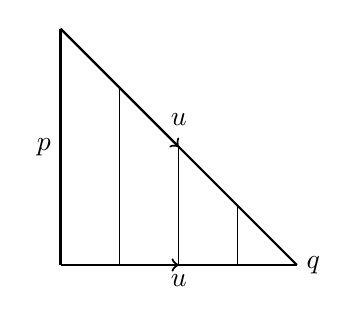
\begin{tikzpicture}[scale = 3]
					\draw [thick] (0,0) -- (1,0);
					\draw [thick] (0,0) -- (0,1);
					\draw [thick] (0,1) -- (1,0);
					\draw [thick,->] (0,0) -- (.5,0);
					\draw [thick,->] (0,1) -- (.5,.5);
				
					\draw [thin] (.25,0) -- (.25,.75);
					\draw [thin] (.5,0) -- (.5,.5);
					\draw [thin] (.75,0) -- (.75,.25);

					\draw (.5,0) node[below] {$u$};
					\draw (.5,.55) node[above] {$u$};
					\draw (0,.5) node[left] {$p$};
					\draw (1,0) node[right] {$q$};
				\end{tikzpicture}
				\caption{$\langle \wbar{u} \rangle = - \langle u \rangle$.}
				\label{fig:additive_inverse}
			\end{subfigure}
			~
			\begin{subfigure}[b]{.4\textwidth}
				\centering
				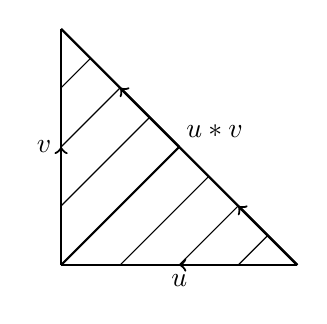
\begin{tikzpicture}[scale = 3]
					\draw [thick] (0,0) -- (1,0);
					\draw [thick] (0,0) -- (0,1);
					\draw [thick] (0,1) -- (1,0);
					\draw [thick] (0,0) -- (.5,.5);
					\draw [thick,->] (1,0) -- (.75,.25);
					\draw [thick,->] (.5,.5) -- (.25,.75);
					\draw [thick,->] (1,0) -- (.5,0);
					\draw [thick,->] (0,0) -- (0,.5);
				
					\draw [thin] (.25,0) -- (.625,.375);
					\draw [thin] (.5,0) -- (.75,.25);
					\draw [thin] (.75,0) -- (.875,.125);

					\draw [thin] (0,.25) -- (.375,.625);
					\draw [thin] (0,.5) -- (.25,.75);
					\draw [thin] (0,.75) -- (.125,.875);

					\draw (.5,0) node[below] {$u$};
					\draw (.65,.5) node[above] {$u \ast v$};
					\draw (0,.5) node[left] {$v$};
				\end{tikzpicture}
				\caption{$\langle u \ast v \rangle = \langle u \rangle + \langle v \rangle$.}
				\label{fig:hurewicz_homomorphism}
			\end{subfigure}
		\end{figure}
	\end{proof}

	\begin{lemma}
		\label{lem:concatenation_addition}
		Let $u$ and $v$ be paths in $X$ from $p$ to $q$ and from $q$ to $r$, respectively. Then $\langle u \ast v \rangle = \langle u \rangle + \langle v \rangle$.	
	\end{lemma}

	\begin{proof}
		Consider figure \ref{fig:hurewicz_homomorphism}. The thin lines correspond to where $y - x$ is constant. Hence define $\sigma : \Delta^2 \to X$ by
		\begin{equation*}
			\sigma(x,y) := \ccases{
				u(y - x + 1) & 0 \leq y \leq x \leq 1,\\
				v(y - x) & 0 \leq x \leq y \leq 1.
			}
		\end{equation*}
		An application of the gluing lemma shows that $\sigma$ is actually a singular $2$-simplex. Moreover
		\begin{equation*}
			\partial \sigma = u \ast v - v + \wbar{u}.
		\end{equation*}
		Hence lemma \ref{lem:reverse_path_homology} yield
		\begin{equation*}
			0 = \langle u \ast v - v + \wbar{u}\rangle = \langle u \ast v \rangle - \langle v \rangle - \langle u \rangle.
		\end{equation*}
	\end{proof}

	\begin{corollary}
		\label{cor:h_homomorphism}
		$h$ is a morphism of groups.
	\end{corollary}

	\begin{corollary}
		\label{cor:composable_associative_homology}
		Let $u,v,w$ be composable paths in $X$. Then $\langle (u \ast v) \ast w \rangle = \langle u \ast (v \ast w) \rangle$.
	\end{corollary}

	\begin{lemma}
		$h$ is surjective.
	\end{lemma}

	\begin{proof}
		Let $x \in X$. If $x = p$, define $\gamma_p := c_p$. If $x \neq p$, by the path connectedness of $X$ we can choose a path $\gamma_x$ from $p$ to $x$. Hence we get a map $\gamma : X \to \mathsf{Top}(\Delta^1,X)$. Extending by linearity yields a mapping $\gamma : C_0(X) \to C_1(X)$. Let $c := \sum_{k = 1}^n m_k \sigma_k$ be a $1$-cycle in $X$. Consider
		\begin{equation*}
			\sbr{u} := \sbr[0]{\gamma_{\sigma_1(0)} \ast \sigma_1 \ast \overline{\gamma_{\sigma_1(1)}}}^{m_1} \cdots \sbr[0]{\gamma_{\sigma_n(0)} \ast \sigma_n \ast \overline{\gamma_{\sigma_n(1)}}}^{m_n} \in \pi_1(X,p). 
		\end{equation*}
		Now lemma \ref{lem:reverse_path_homology} and \ref{lem:concatenation_addition}, corollary \ref{cor:h_homomorphism} and \ref{cor:composable_associative_homology} yields
		\begin{align*}
			h(\sbr{u}) &= \sum_{k = 1}^n m_k \langle\gamma_{\sigma_k(0)} \ast \sigma_k \ast \overline{\gamma_{\sigma_k(1)}}\rangle\\
			&= \sum_{k = 1}^n m_k \del[1]{\langle\gamma_{\sigma_k(0)}\rangle + \langle\sigma_k\rangle + \langle \overline{\gamma_{\sigma_k(1)}}\rangle}\\
			&= \sum_{k = 1}^n m_k \del[1]{\langle\gamma_{\sigma_k(0)}\rangle + \langle\sigma_k\rangle - \langle \gamma_{\sigma_k(1)}}\rangle\\
			&= \langle c \rangle - \sum_{k = 1}^n m_k \langle \gamma_{\sigma_k(1) - \sigma_k(0)}\rangle\\
			&= \langle c \rangle - \sum_{k = 1}^n m_k \langle \gamma_{\partial \sigma_k}\rangle\\
			&= \langle c \rangle - \langle \gamma_{\partial c}\rangle\\
			&= \langle c \rangle.
		\end{align*}
	\end{proof}

	Lastly, we want to show that $\ker h = \sbr[0]{\pi_1(X,p),\pi_1(X,p)}$. Since then the first isomorphism theorem implies $\Ab(\pi_1(X,p)) \cong H_1(X)$. Since $H_1(X)$ is abelian, clearly $\sbr[0]{\pi_1(X,p),\pi_1(X,p)} \subseteq \ker h$ and thus $h$ factors uniquely $\wtilde{h} : \Ab(\pi_1(X,p)) \to H_1(X)$. The next lemma will be useful.
	
	\begin{lemma}
		\label{lem:nullhomotopic_loop}
		Let $\sigma : \Delta^2 \to X$ be a singular $2$-simplex. Define $\sigma^{(k)} := \sigma \circ \varphi^2_k$ for $k = 0,1,2$. Then $\sbr[0]{\sigma^{(0)} \ast \overline{\sigma^{(1)}} \ast \sigma^{(2)}} = \sbr[0]{c_{\sigma(e_1)}}$.
	\end{lemma}

	\begin{proof}
		Let $u := \sigma^{(0)} \ast \overline{\sigma^{(1)}} \ast \sigma^{(2)}$. Since $\mathbb{B}^2 \approx \Delta^2$, we can consider $\sigma : \mathbb{B}^2 \to X$. One can check that the circle representative $\wtilde{u}$ of $u$ is the reparametrized restriction $\sigma \vert_{\mathbb{S}^1}$. Since reparametrizations are invariant under homotopies, we have that $u$ is a nullhomotopic loop.
	\end{proof}

	Let $\sigma \in \mathsf{Top}(\Delta^1,X)$. Define $g(\sigma) := \sbr[0]{\gamma_{\sigma(0)} \ast \sigma \ast \overline{\gamma_{\sigma(1)}}}_{\Ab}$, where $\sbr{u}_{\Ab}$ denotes the equivalence class of $\sbr{u}$ in $\Ab(\pi_1(X,p))$. Since $\Ab(\pi_1(X,p))$ is abelian, extension by linearity yields a map $g : C_1(X) \to \Ab(\pi_1(X,p))$.

	\begin{lemma}
		\label{lem:g_vanishes_on_boundaries}
		$g$ vanishes on $\im \partial_2$.	
	\end{lemma}

	\begin{proof}
		Let $\sigma \in \mathsf{Top}(\Delta^2,X)$. Then lemma \ref{lem:nullhomotopic_loop} yields
		\begin{align*}
			g(\partial \sigma) &= g\del[1]{\sigma^{(0)}} g\del[1]{\sigma^{(1)}}^{-1}g\del[1]{\sigma^{(2)}}\\
			&= \sbr[1]{\gamma_{\sigma(e_1)} \ast \sigma^{(0)} \ast \overline{\gamma_{\sigma(e_2)}} \ast \gamma_{\sigma(e_2)} \ast \overline{\sigma^{(1)}} \ast \overline{\gamma_{\sigma(e_0)}} \ast \gamma_{\sigma(e_0)} \ast \sigma^{(2)} \ast \overline{\gamma_{\sigma(e_1)}}}_{\Ab}\\
			&= \sbr[1]{\gamma_{\sigma(e_1)} \ast \sigma^{(0)} \ast \overline{\sigma^{(1)}} \ast \sigma^{(2)} \ast \overline{\gamma_{\sigma(e_1)}}}_{\Ab}\\
			&= \sbr[1]{\gamma_{\sigma(e_1)} \ast c_{\sigma(e_1)} \ast \overline{\gamma_{\sigma(e_1)}}}_{\Ab}\\
			&= \sbr{c_p}_{\Ab}.
		\end{align*}
	\end{proof}

	By lemma \ref{lem:g_vanishes_on_boundaries}, $g$ passes to the quotient and yields a map $\wtilde{g} : H_1(X) \to \Ab(\pi_1(X,p))$. Moreover
	\begin{equation*}
		(\wtilde{g} \circ \wtilde{h})\sbr{u}_{\Ab} = \wtilde{g}\del[1]{h\sbr{u}} = \wtilde{g}\langle u \rangle = g(u) = \sbr[0]{c_p \ast u \ast \overline{c_p}}_{\Ab} = \sbr{u}_{\Ab}
	\end{equation*}
	\noindent and thus $\wtilde{h}$ admits a retraction in $\mathsf{AbGrp}$ which implies that $\wtilde{h}$ is injective. Hence $\ker \wtilde{h}$ is trivial and thus if we write $\pi : \pi_1(X,p) \to \Ab(\pi_1(X,p))$ for the canoncial projection
	\begin{equation*}
		\ker h = \ker(\wtilde{h} \circ \pi) = (\wtilde{h} \circ \pi)^{-1}(0) = \pi^{-1}\del[1]{\wtilde{h}^{-1}(0)} = \pi^{-1}(0) = \sbr[0]{\pi_1(X,p),\pi_1(X,p)}. 
	\end{equation*}	
\end{proof}

\begin{definition}[Hurewicz Homomorphism]
	Let $X \in \ob(\mathsf{Top})$ and $p \in X$. The homomorphism $h : \pi_1(X,p) \to H_1(X)$ defined in theorem \ref{thm:Hurewicz_theorem} is called the \bld{Hurewicz homomorphism}.
\end{definition}

\begin{proposition}
	Let $U : \mathsf{AbGrp} \to \mathsf{Grp}$ denote the forgetful functor. Then the Hurewicz homomorphism is a natural transformation $\pi_1 \Rightarrow U \circ H_1$.
\end{proposition}

\begin{proof}
	
\end{proof}

%%%%%%%%%%%%%%%%%%%%%%%%%%%%%%%%%%%%%%%%%%%%%%%%%%%%%%%%%%%%%%%%%%%%%%%%%%%%%%%%%%%%%%%%%%%%%%%%%%%%%%%%%%%%%
%																							%
%%%%%%%%%%%%%%%%%%%%%%%%%%%%%%%%%%%%%%%%%%%%%%%%%%%%%%%%%%%%%%%%%%%%%%%%%%%%%%%%%%%%%%%%%%%%%%%%%%%%%%%%%%%%%
\section*{Barycentric Subdivision}



\section*{Applications}
\subsection*{$\mathbb{S}^n$ is not contractible}

\begin{definition}[Retract]
	Let $X \in \ob(\mathsf{Top})$ and $S \subseteq X$ a subspace. We say that \bld{$S$ is a retract of $X$},  if the inclusion $\iota : S \hookrightarrow X$ admits a retraction in $\mathsf{Top}$.
\end{definition}

\begin{lemma}
	Let $n \in \mathbb{Z}$, $n \geq 1$. Then $\mathbb{S}^n$ is not a retract of $\mathbb{B}^{n + 1}$. 	
\end{lemma}

\begin{proof}
	
\end{proof}

\begin{proposition}
	Let $n \in \omega$, $X \in \ob(\mathsf{Top})$ and $f \in \mathsf{Top}(\mathbb{S}^n,X)$. Then the followin conditions are equivalent:
	\begin{enumerate}[label = \textup{(}\alph*\textup{)},wide = 0pt]
		\item $f$ is nullhomotopic.
		\item $f$ admits a continuous extension to $\mathbb{B}^{n+1}$.
		\item Let $p \in \mathbb{S}^n$. Then $f \simeq_p c_{f(p)}$.
	\end{enumerate}
\end{proposition}

\begin{proof}
	We show (a)$\Rightarrow$(b)$\Rightarrow$(c)$\Rightarrow$(a). Assume that (a) holds. Hence we have that $H : f \simeq c_p$ for some $p \in X$. Define $g : \mathbb{B}^{n+1} \to X$ by
	\begin{equation*}
		g(x) := \ccases{
			p & 0 \leq \abs{x} \leq \frac{1}{2},\\
			H(x/\abs{x},2 - 2 \abs{x}) & \frac{1}{2} \leq \abs{x} \leq 1.
		}
	\end{equation*}
	Then $g \in \mathsf{Top}(\mathbb{B}^{n+1},X)$ by the gluing lemma and $g\vert_{\mathbb{S}^n} = f$. Assume that (b) holds. So let $g \in \mathsf{Top}(\mathbb{B}^{n+1},X)$ be an extension of $f$. Define $H : \mathbb{S}^n \times I \to X$ by
	\begin{equation*}
		H(x,t) := g((1 - t)x + tp,t).
	\end{equation*}
	Then it is easy to check that $H : f \simeq_p c_{f(p)}$. Finally, (c)$\Rightarrow$(a) is immediate.
\end{proof}

\subsection*{The Brouwer Fixed Point Theorem}
\begin{theorem}[Brouwer Fixed Point Theorem]
	Let $n \in \mathbb{Z}$, $n \geq 1$. Then every mapping $f \in \mathsf{Top}(\mathbb{B}^n,\mathbb{B}^n)$ has a fixed point.	
	\label{thm:brouwer_fixed_point}
\end{theorem}

\begin{proof}
	
\end{proof}
